\documentclass[11pt,a4paper]{article}

\usepackage[margin=2.2cm]{geometry}
\usepackage[T1]{fontenc}
\usepackage{lmodern}
\usepackage{microtype}
\usepackage{amsmath,amssymb}
\usepackage{booktabs}
\usepackage{array}
\usepackage{graphicx}
\usepackage{caption}
\usepackage{subcaption}
\usepackage{xcolor}
\usepackage{listings}
\usepackage{tikz}
\usetikzlibrary{arrows.meta,positioning,angles,quotes,calc}
\usepackage{enumitem}
\usepackage{siunitx}
\usepackage[hidelinks]{hyperref}

\setlist{itemsep=2pt,topsep=3pt}
\captionsetup{font=small,labelfont=bf}
\graphicspath{{figures/}{images/}}

% ---------------------------------------------------------------------------
\definecolor{codebg}{RGB}{247,247,247}
\definecolor{codekw}{RGB}{0,72,153}
\definecolor{codecm}{RGB}{110,110,110}
\definecolor{codestr}{RGB}{163,21,21}
\lstset{
  language=Python,
  basicstyle=\ttfamily\footnotesize,
  keywordstyle=\color{codekw}\bfseries,
  commentstyle=\color{codecm}\itshape,
  stringstyle=\color{codestr},
  backgroundcolor=\color{codebg},
  frame=single, rulecolor=\color{black!25},
  numbers=left, numberstyle=\tiny\color{black!50}, numbersep=6pt,
  breaklines=true, breakatwhitespace=true,
  showstringspaces=false, columns=fullflexible, keepspaces=true,
  xleftmargin=1.6em, framexleftmargin=1.4em,
  aboveskip=6pt, belowskip=6pt,
  inputencoding=utf8, extendedchars=true,
  literate={π}{{$\pi$}}1 {—}{{---}}1,
}
\newcommand{\src}{../src/gp7_pick_place/gp7_pick_place}

% ---------------------------------------------------------------------------
\newcommand{\cs}[1]{c_{#1}}
\newcommand{\sn}[1]{s_{#1}}
\newcommand{\atantwo}{\operatorname{atan2}}
\newcommand{\R}[2]{\mathbf{R}^{#1}_{#2}}
\newcommand{\T}[2]{\mathbf{T}^{#1}_{#2}}

\newcommand{\repo}{\url{https://github.com/Lasan-Perera/6DoF-Robot-Manipulator-Simulation}}
\newcommand{\videolink}{\url{https://youtu.be/XFLGYKSj5Rc}}

\begin{document}

% =========================================================================
\begin{center}
  {\LARGE\bfseries EN3563 -- Robotics}\\[4pt]
  {\Large Mini Project: Pick-and-Place with a Yaskawa GP7 in Gazebo}\\[10pt]
  \begin{tabular}{ll}
    \toprule
    \textbf{Name} & \textbf{Index number} \\
    \midrule
    Perera W.A.L.S & 230487D \\
    Priyadarshana S.A.D & 230502X \\
    \bottomrule
  \end{tabular}\\[8pt]
  \small GitHub: \repo\\
  Video: \videolink
\end{center}

% =========================================================================
\section{System overview}

\begin{figure}[h]
\centering
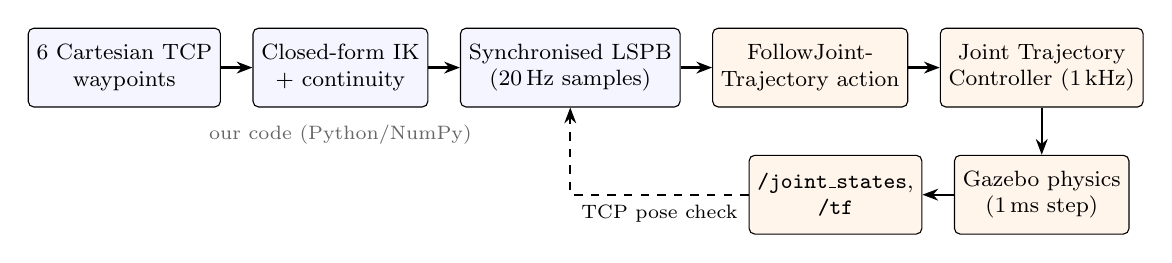
\begin{tikzpicture}[
  node distance=4mm,
  blk/.style={draw, rounded corners=2pt, align=center, font=\footnotesize,
              minimum height=10mm, inner sep=3pt, fill=blue!4},
  ros/.style={blk, fill=orange!8},
  arr/.style={-{Stealth[length=2mm]}, thick}]
  \node[blk] (wp) {6 Cartesian TCP\\waypoints};
  \node[blk, right=of wp] (ik) {Closed-form IK\\+ continuity};
  \node[blk, right=of ik] (tr) {Synchronised LSPB\\(20\,Hz samples)};
  \node[ros, right=of tr] (ac) {FollowJoint-\\Trajectory action};
  \node[ros, right=of ac] (jtc) {Joint Trajectory\\Controller (1\,kHz)};
  \node[ros, below=6mm of jtc] (gz) {Gazebo physics\\(1\,ms step)};
  \node[ros, left=of gz] (js) {\texttt{/joint\_states},\\ \texttt{/tf}};
  \draw[arr] (wp) -- (ik); \draw[arr] (ik) -- (tr); \draw[arr] (tr) -- (ac);
  \draw[arr] (ac) -- (jtc); \draw[arr] (jtc) -- (gz); \draw[arr] (gz) -- (js);
  \draw[arr, dashed] (js.west) -| node[pos=0.25, below, font=\scriptsize]{TCP pose check} (tr.south);
  \node[font=\scriptsize, text=black!60, below=1mm of ik] {our code (Python/NumPy)};
\end{tikzpicture}
\caption{Software pipeline. Blue: our code. Orange: ROS~2 / \texttt{ros2\_control} / Gazebo.}
\label{fig:pipeline}
\end{figure}

The work is split into two ROS~2 packages. \texttt{gp7\_description} holds the robot
model, worlds, launch files and controller configuration. \texttt{gp7\_pick\_place}
holds all the mathematics (\texttt{kinematics.py}, \texttt{trajectory.py},
\texttt{jacobian.py}, \texttt{singularity.py}) and the mission node
\texttt{run\_pick\_place.py} (Fig.~\ref{fig:pipeline}).

% =========================================================================
\section{Simulation setup in Gazebo}

\paragraph{Robot model.}
The arm's link geometry, joint origins, axes and limits come from the ROS-Industrial
\texttt{motoman\_gp7\_support} package~\cite{rosi}, which is generated from Yaskawa's
CAD data. We ported it from ROS~1 to ROS~2. Link lengths were checked against
the datasheet drawing and the GP7 specification~\cite{gp7spec}. The source model has no
inertial data, which Gazebo needs for dynamics. We therefore computed each link's
volume, centre of mass and inertia tensor from its mesh and scaled all masses uniformly
so that they add up to the published robot mass of \SI{34}{kg}. A Robotiq 2F-85
gripper~\cite{robotiq} is mounted on \texttt{tool0}. We define the tool centre point
(TCP) \(L_\text{TCP}=\SI{0.112}{m}\) along \texttt{tool0}'s approach axis, between the
finger pads.

\paragraph{Physics and control.}
Gazebo Harmonic runs with a 1\,ms step. The 2F-85 is an under-actuated linkage with one
driven knuckle joint and five \emph{mimic} joints. Gazebo's default DART engine does not
enforce mimic constraints (the fingers hung asymmetrically), so we use the
\textbf{bullet-featherstone} engine. The \texttt{gz\_ros2\_control} plugin
runs a controller manager at 1\,kHz with a \texttt{JointTrajectoryController} for the six
arm joints, another for the gripper knuckle, and a \texttt{joint\_state\_broadcaster}.

\paragraph{Environment.}
Table~\ref{tab:world} lists the scene (\texttt{worlds/pick\_place.sdf}).
\begin{table}[h]
\centering\small
\begin{tabular}{lll}
\toprule
Object & Size & Position (centre of base, m) \\
\midrule
GP7 robot & -- & \((0, 0, 0)\) \\
Box A (static) & \(0.30\times0.30\times0.20\) m & \((0.5, 0.5, 0)\) \;-- top surface at \(z=0.20\) \\
Box B (dynamic, 0.1 kg) & \(0.05\times0.05\times0.05\) m & \((0.55, -0.25, 0)\) \;-- on the ground \\
\bottomrule
\end{tabular}
\caption{Simulation environment.}
\label{tab:world}
\end{table}

\paragraph{Why Box~A is not at \((1,1,0)\).}
The task sheet places Box~A at \((1, 1, 0)\), which is \(\sqrt2 = \SI{1.414}{m}\) from the
base axis. To place Box~B with the gripper pointing down, the wrist centre must lie
directly above the placement point, so its horizontal distance from the base axis would be
\SI{1.414}{m}. The largest horizontal wrist-centre distance the GP7 can reach is
\(a_1 + a_2 + \sqrt{a_3^2+d_4^2} = 0.040 + 0.445 + 0.442 = \SI{0.927}{m}\), which matches
Yaskawa's published reach of \SI{927}{mm}. The box at \((1,1)\) is therefore out of reach
for any IK branch and any gripper. We kept Box~A's dimensions and moved it to
\((0.5, 0.5, 0)\), keeping the same \(45^\circ\) direction from the base.
Box~B was placed at \((0.55,-0.25,0)\), a reachable ground position we chose. Its pick
coordinates are the only scene-dependent inputs of the mission node.

% =========================================================================
\section{Coordinate frames and D-H parameters}

We use the standard (distal) Denavit--Hartenberg convention: joint \(i\) rotates about
\(z_{i-1}\), and
\begin{equation}
\mathbf A_i = \mathrm{Rot}_{z}(\theta_i)\,\mathrm{Trans}_{z}(d_i)\,\mathrm{Trans}_{x}(a_i)\,\mathrm{Rot}_{x}(\alpha_i)
=\begin{bmatrix}
\cs{\theta_i} & -\sn{\theta_i}\cs{\alpha_i} & \sn{\theta_i}\sn{\alpha_i} & a_i\cs{\theta_i}\\
\sn{\theta_i} & \cs{\theta_i}\cs{\alpha_i} & -\cs{\theta_i}\sn{\alpha_i} & a_i\sn{\theta_i}\\
0 & \sn{\alpha_i} & \cs{\alpha_i} & d_i\\
0&0&0&1\end{bmatrix}.
\label{eq:dh}
\end{equation}
Fig.~\ref{fig:frames} shows the frame assignment at the zero pose: upper arm vertical,
forearm horizontal along world \(+X\). Axes 4, 5 and 6 intersect at one point (a spherical
wrist), so \(o_4 \equiv o_5\) is the \emph{wrist centre}.

\begin{figure}[t]
\centering
\begin{subfigure}[b]{0.50\textwidth}\centering
  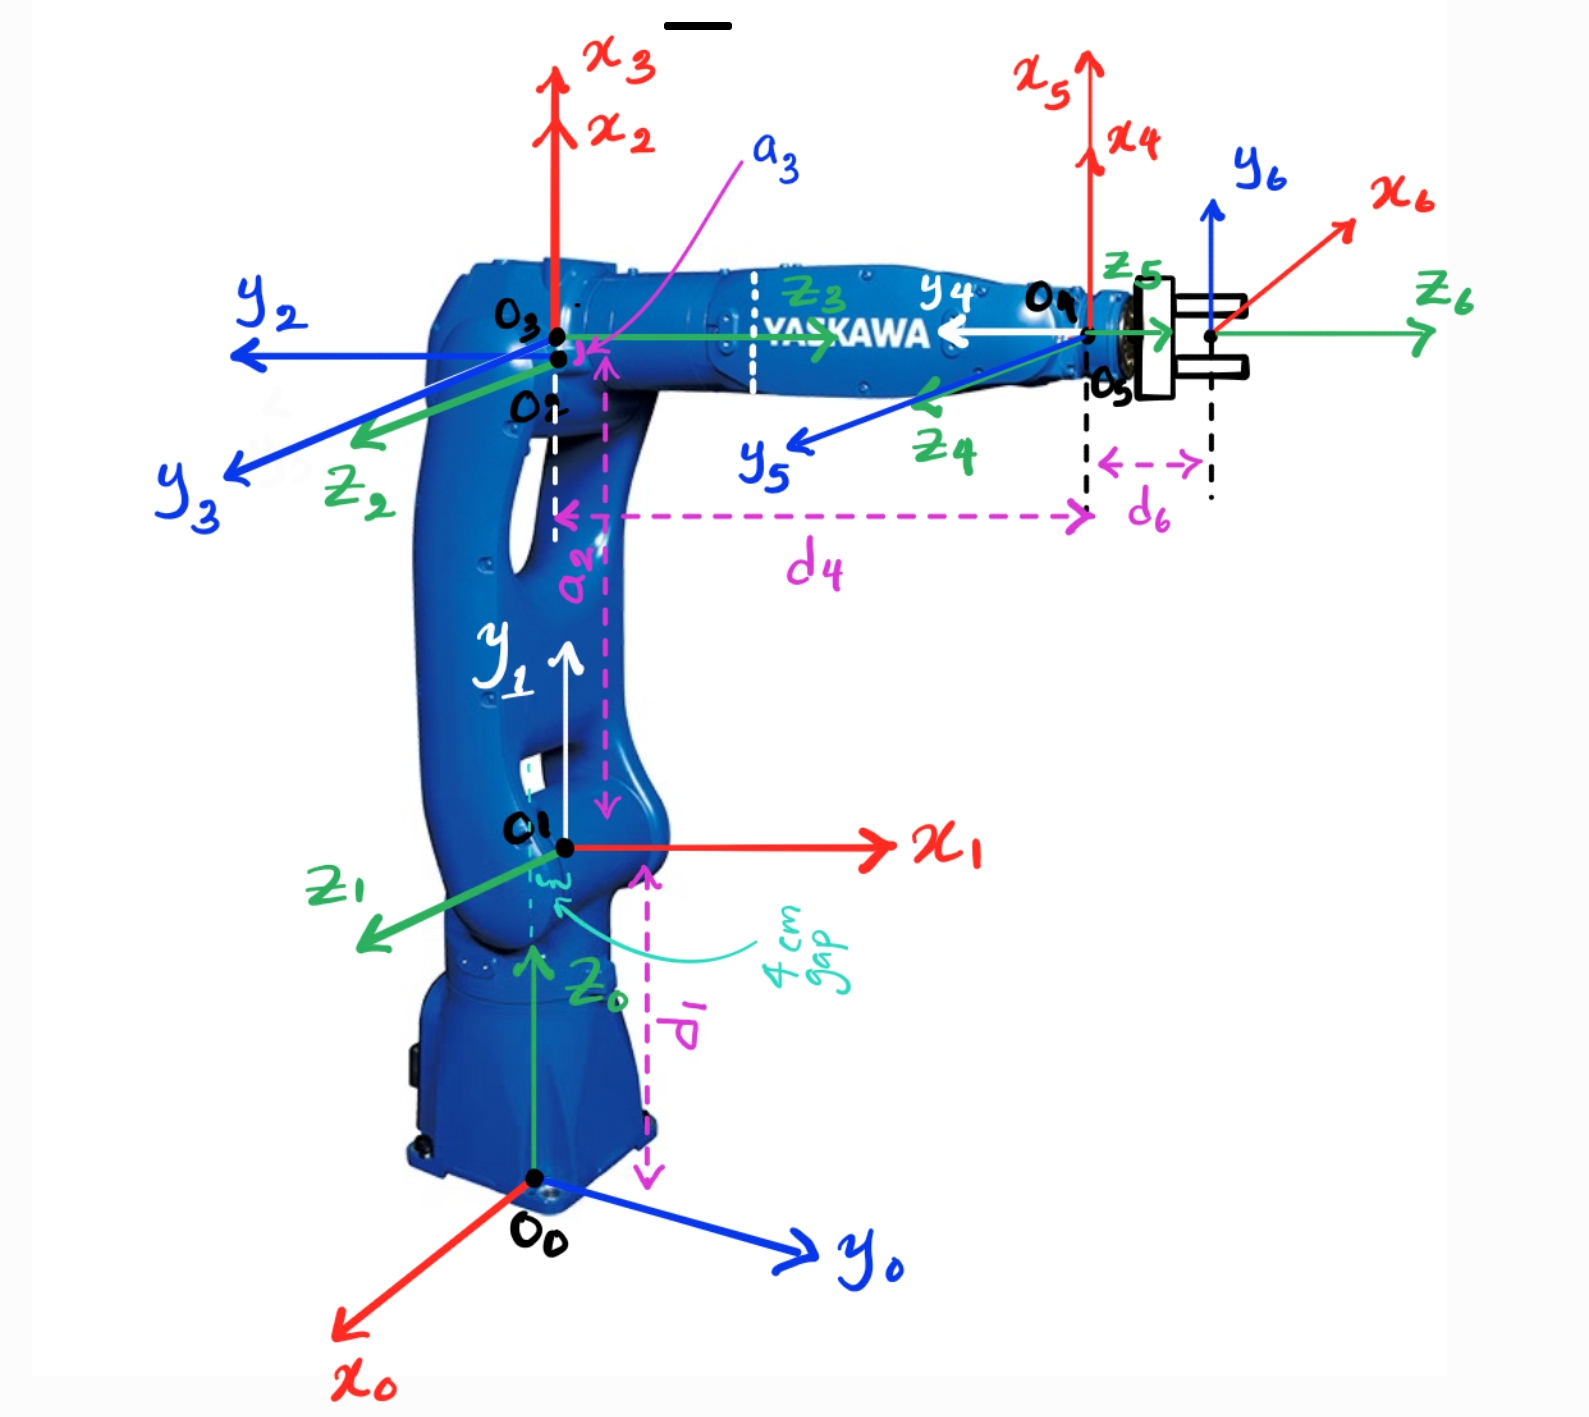
\includegraphics[width=\linewidth]{dh-frames.jpg}
  \caption{Hand-drawn frames on the GP7 at its zero pose.}
\end{subfigure}\hfill
\begin{subfigure}[b]{0.47\textwidth}\centering
  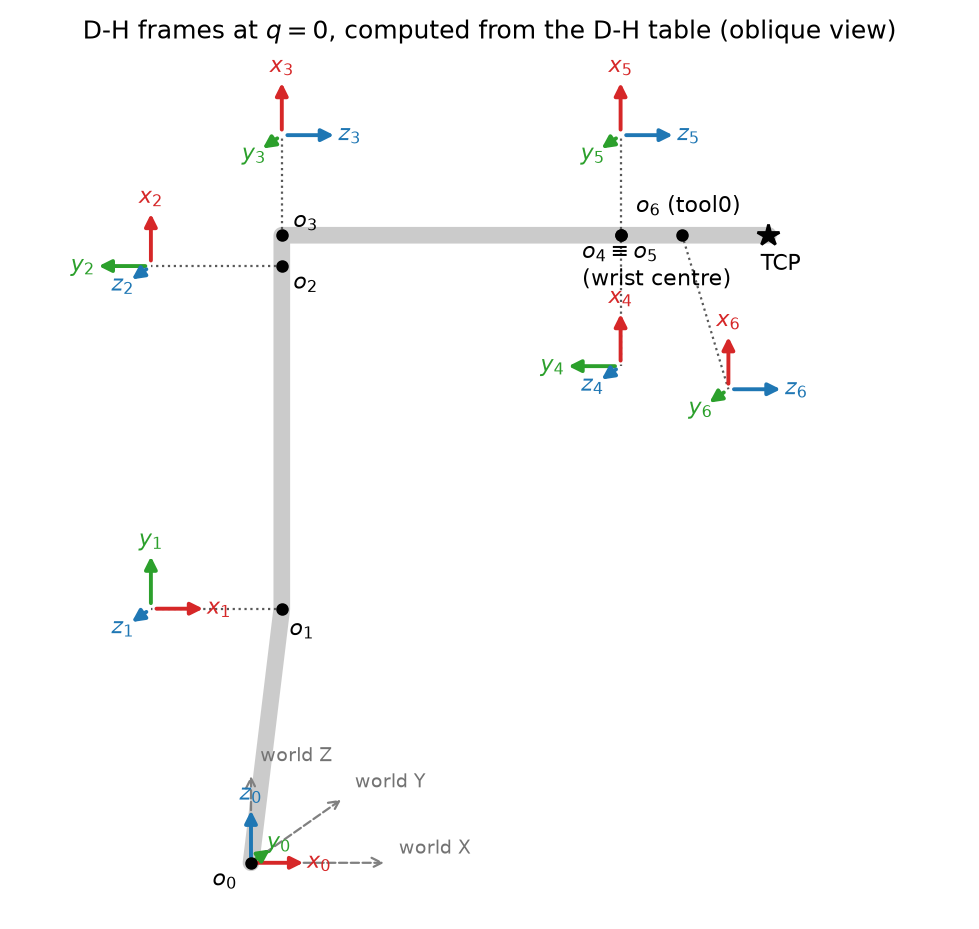
\includegraphics[width=\linewidth]{frames_zero_pose.png}
  \caption{Frames computed from Table~\ref{tab:dh} (\(q=0\)).}
\end{subfigure}
\caption{Coordinate frame assignment. In (b), triads whose origins coincide or nearly
coincide are drawn offset and joined to their origin by a dotted line. At \(q=0\)
the D-H rules give \(x_0 \parallel x_1\) (world \(+X\)) and \(x_6 \parallel x_5\)
(world \(+Z\), since \(\alpha_6=0\)). Panel (b) is computed directly from the D-H matrices
and is authoritative where the sketch differs.}
\label{fig:frames}
\end{figure}

\begin{table}[h]
\centering\small
\begin{tabular}{c S[table-format=1.3] r S[table-format=1.3] l l}
\toprule
\(i\) & {\(a_i\) (m)} & \(\alpha_i\) & {\(d_i\) (m)} & \(\theta_i\) (in terms of joint angle \(q_i\)) & Physical meaning \\
\midrule
1 & 0.040 & \(90^\circ\)  & 0.330 & \(q_1\)              & base height; 40\,mm shoulder offset \\
2 & 0.445 & \(0^\circ\)   & 0     & \(90^\circ - q_2\)   & upper arm (axes 2, 3 parallel) \\
3 & 0.040 & \(90^\circ\)  & 0     & \(q_3\)              & 40\,mm elbow offset \\
4 & 0     & \(-90^\circ\) & 0.440 & \(-q_4\)             & forearm, along the roll axis \\
5 & 0     & \(90^\circ\)  & 0     & \(q_5\)              & wrist bend \\
6 & 0     & \(0^\circ\)   & 0.080 & \(-q_6\)             & wrist centre to flange (\texttt{tool0}) \\
\bottomrule
\end{tabular}
\caption{D-H parameters of the GP7. \(q_i\) are the physical joint angles used by the
controllers. Their zero and positive direction come from the URDF.}
\label{tab:dh}
\end{table}

\paragraph{Joint-angle conventions.}
The D-H axes \(z_1, z_3, z_5\) point opposite to the URDF rotation axes of joints 2, 4 and 6,
so those angles change sign. In addition, the D-H zero of joint 2 (upper arm horizontal) is
\(90^\circ\) from the physical zero (upper arm vertical). Hence
\(\boldsymbol\theta = (q_1,\; 90^\circ - q_2,\; q_3,\; -q_4,\; q_5,\; -q_6)\).
We found these conventions by comparing our FK with Gazebo's TF tree. The \(90^\circ\)
offset showed up at \(q = 0\); the sign of \(\theta_4\) showed up at a general joint
vector. The sign of \(\theta_6\) only affects orientation, so it was found by comparing
full \(4\times4\) transforms. The D-H values agree with an independently published
table for this robot~\cite{dasilva}.

\begin{table}[h]
\centering\small
\begin{tabular}{lcccccc}
\toprule
Joint & 1 (S) & 2 (L) & 3 (U) & 4 (R) & 5 (B) & 6 (T) \\
\midrule
Range (deg) & \(\pm170\) & \(-65\ldots145\) & \(-70\ldots190\) & \(\pm190\) & \(\pm135\) & \(\pm360\) \\
Max speed (deg/s) & 375 & 315 & 410 & 550 & 550 & 1000 \\
\bottomrule
\end{tabular}
\caption{Joint ranges and maximum speeds from the GP7 specification~\cite{gp7spec}.}
\label{tab:limits}
\end{table}

% =========================================================================
\section{Forward kinematics}

Substituting Table~\ref{tab:dh} into~\eqref{eq:dh}, with
\(c_i=\cos\theta_i\), \(s_i=\sin\theta_i\), \(c_{23} = \cos(\theta_2+\theta_3)\):
\begin{gather*}
\mathbf A_1=\begin{bmatrix}c_1&0&s_1&a_1c_1\\ s_1&0&-c_1&a_1s_1\\0&1&0&d_1\\0&0&0&1\end{bmatrix}\!,\;
\mathbf A_2=\begin{bmatrix}c_2&-s_2&0&a_2c_2\\ s_2&c_2&0&a_2s_2\\0&0&1&0\\0&0&0&1\end{bmatrix}\!,\;
\mathbf A_3=\begin{bmatrix}c_3&0&s_3&a_3c_3\\ s_3&0&-c_3&a_3s_3\\0&1&0&0\\0&0&0&1\end{bmatrix}\!,\\[4pt]
\mathbf A_4=\begin{bmatrix}c_4&0&-s_4&0\\ s_4&0&c_4&0\\0&-1&0&d_4\\0&0&0&1\end{bmatrix}\!,\;
\mathbf A_5=\begin{bmatrix}c_5&0&s_5&0\\ s_5&0&-c_5&0\\0&1&0&0\\0&0&0&1\end{bmatrix}\!,\;
\mathbf A_6=\begin{bmatrix}c_6&-s_6&0&0\\ s_6&c_6&0&0\\0&0&1&d_6\\0&0&0&1\end{bmatrix}\!.
\end{gather*}
The flange pose is \(\T{0}{6}=\mathbf A_1\mathbf A_2\cdots\mathbf A_6\) and the TCP pose is
\(\T{0}{\text{TCP}} = \T{0}{6}\,\mathrm{Trans}_z(L_\text{TCP})\). The \(\mathbf R^0_6\) of the TCP
is the same as that of \texttt{tool0}. Multiplying out the first four transforms (we checked
the result symbolically with SymPy) gives the closed forms used by the inverse kinematics:
\begin{align}
\mathbf o_c = \mathbf o_4 &=
\begin{bmatrix}
\big(a_1 + a_2c_2 + a_3c_{23} + d_4 s_{23}\big)\,c_1\\
\big(a_1 + a_2c_2 + a_3c_{23} + d_4 s_{23}\big)\,s_1\\
d_1 + a_2 s_2 + a_3 s_{23} - d_4 c_{23}
\end{bmatrix}, &
\R{0}{3} &= \begin{bmatrix}
c_1c_{23} & s_1 & c_1 s_{23}\\
s_1c_{23} & -c_1 & s_1 s_{23}\\
s_{23} & 0 & -c_{23}\end{bmatrix},
\label{eq:fkpos}
\end{align}
\begin{equation}
\R{3}{6} = \begin{bmatrix}
c_4c_5c_6 - s_4s_6 & -c_4c_5s_6 - s_4c_6 & c_4 s_5\\
s_4c_5c_6 + c_4s_6 & -s_4c_5s_6 + c_4c_6 & s_4 s_5\\
-s_5c_6 & s_5 s_6 & c_5\end{bmatrix},
\qquad
\mathbf p_{6} = \mathbf o_c + d_6\,\mathbf z_6 .
\label{eq:r36}
\end{equation}
At \(q=0\) (\(\boldsymbol\theta = (0,90^\circ,0,0,0,0)\)), Eq.~\eqref{eq:fkpos} gives
\(\mathbf o_c = (0.480, 0, 0.815)\), \(\mathbf p_6 = (0.560, 0, 0.815)\) and the TCP at
\((0.672, 0, 0.815)\)\,m. These match the sums of the URDF joint offsets.

\paragraph{Verification.}
We compared the FK with Gazebo's live transform (\texttt{tf2\_echo base\_link tool0}),
Table~\ref{tab:fkcheck}. Over 20 random joint vectors, the full \(4\times4\) transforms
also matched \texttt{robot\_state\_publisher} with a largest residual of
\(5\times10^{-13}\)\,mm and \(7\times10^{-14}\,^\circ\).
\begin{table}[h]
\centering\small
\begin{tabular}{lcc}
\toprule
\(q\) (rad) & FK \texttt{tool0} position (m) & Gazebo TF (m) \\
\midrule
\((0,0,0,0,0,0)\) & \((0.560, 0.000, 0.815)\) & \((0.560, 0.000, 0.815)\) \\
\((0.3, 0.2, -0.1, 0.4, 0.15, 0.2)\) & \((0.6095, 0.1934, 0.6615)\) & \((0.609, 0.193, 0.661)\) \\
\((-0.4,-0.25,0.3,-0.5,0.35,-0.2)\) & \((0.3040, -0.1428, 1.0851)\) & \((0.304, -0.143, 1.085)\) \\
\bottomrule
\end{tabular}
\caption{Forward kinematics compared with the simulator.}
\label{tab:fkcheck}
\end{table}

% =========================================================================
\section{Inverse kinematics}

Because the GP7 has a spherical wrist (Pieper's condition), the problem decouples:
joints 1--3 position the wrist centre, and joints 4--6 set the orientation.

\paragraph{Step 1: wrist centre.}
For a desired TCP pose \((\mathbf p, \mathbf R)\), step back along the approach axis
\(\mathbf z = \mathbf R_{:,3}\) by the gripper length plus the flange distance:
\begin{equation}
\mathbf o_c = (x_c, y_c, z_c) = \mathbf p - (L_\text{TCP} + d_6)\,\mathbf R\,\hat{\mathbf k}
= \mathbf p - 0.192\,\mathbf R_{:,3}.
\end{equation}

\paragraph{Step 2: position joints \(q_1, q_2, q_3\).}
From Eq.~\eqref{eq:fkpos}, \(\mathbf o_c\) lies in the vertical plane at azimuth \(\theta_1\), so
\begin{equation}
q_1 = \atantwo(y_c,\, x_c) \qquad(\text{second solution } q_1+\pi).
\end{equation}
In that plane (Fig.~\ref{fig:ikplane}) we measure from the shoulder axis \(o_1\):
\(r = \sqrt{x_c^2+y_c^2} - a_1\) and \(s = z_c - d_1\). The elbow-to-wrist-centre link
has effective length \(\ell = \sqrt{a_3^2 + d_4^2} = \SI{0.4418}{m}\) and is inclined
at \(\phi=\atantwo(a_3,d_4) = 5.19^\circ\) to the forearm because of the 40\,mm elbow offset.
With \(L=\sqrt{r^2+s^2}\), the law of cosines gives
\begin{equation}
\alpha = \atantwo(s, r),\quad
\beta = \arccos\frac{a_2^2 + L^2 - \ell^2}{2a_2L},\quad
\gamma = \arccos\frac{a_2^2 + \ell^2 - L^2}{2a_2\ell}.
\end{equation}
The upper arm's elevation is \(\theta_2 = \alpha+\beta\) (elbow up) or \(\alpha-\beta\)
(elbow down). Converting to the physical joint angles:
\begin{equation}
\begin{aligned}
\text{elbow up:}&\quad q_2 = 90^\circ - (\alpha+\beta), & q_3 &= \gamma - \phi - 90^\circ,\\
\text{elbow down:}&\quad q_2 = 90^\circ - (\alpha-\beta), & q_3 &= -\gamma - \phi - 90^\circ.
\end{aligned}
\end{equation}
Check at \(q=0\): \(\mathbf o_c=(0.48,0,0.815)\), so \(r=0.44\), \(s=0.485\),
\(\alpha=47.79^\circ\), \(\beta=42.21^\circ\) and \(\gamma=95.19^\circ = 90^\circ+\phi\).
This gives \(q_2=q_3=0\), as expected.

\begin{figure}[h]
\centering
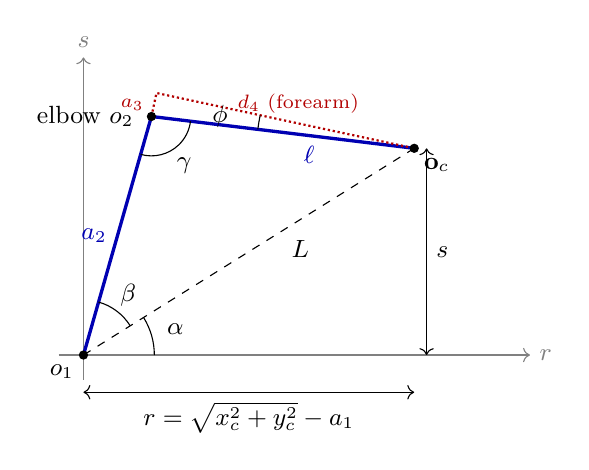
\begin{tikzpicture}[scale=1.05, font=\small]
  \coordinate (O) at (0,0);
  \coordinate (E) at (0.822,2.885);
  \coordinate (W) at (4,2.5);
  \coordinate (H) at (5.2,0);
  \draw[->, gray] (-0.3,0) -- (5.4,0) node[right]{\(r\)};
  \draw[->, gray] (0,-0.3) -- (0,3.6) node[above]{\(s\)};
  \draw[very thick, blue!70!black] (O) -- node[left]{\(a_2\)} (E);
  \draw[very thick, blue!70!black] (E) -- node[below, pos=0.6]{\(\ell\)} (W);
  \draw[dashed] (O) -- node[below right, pos=0.6]{\(L\)} (W);
  \coordinate (M) at (0.883,3.169);
  \draw[densely dotted, thick, red!70!black] (E) -- node[left, font=\scriptsize]{\(a_3\)} (M) -- node[above, font=\scriptsize, pos=0.55]{\(d_4\) (forearm)} (W);
  \fill (O) circle (1.6pt) node[below left]{\(o_1\)};
  \fill (E) circle (1.6pt) node[left=3pt]{elbow \(o_2\)};
  \fill (W) circle (1.6pt) node[below right]{\(\mathbf o_c\)};
  \pic[draw, "\(\alpha\)", angle eccentricity=1.35, angle radius=9mm] {angle = H--O--W};
  \pic[draw, "\(\beta\)", angle eccentricity=1.35, angle radius=7mm] {angle = W--O--E};
  \pic[draw, "\(\gamma\)", angle eccentricity=1.5, angle radius=5mm] {angle = O--E--W};
  \pic[draw, "\(\phi\)", angle eccentricity=1.25, angle radius=20mm] {angle = M--W--E};
  \draw[<->] (4.15,0) -- node[right]{\(s\)} (4.15,2.5);
  \draw[<->] (0,-0.45) -- node[below]{\(r=\sqrt{x_c^2+y_c^2}-a_1\)} (4,-0.45);
\end{tikzpicture}
\caption{Arm plane for \(q_2, q_3\) (elbow-up branch, drawn to scale). The elbow reaches the
wrist centre through the offset \(a_3\) and the forearm \(d_4\), so the straight elbow-to-wrist
line \(\ell\) is inclined by \(\phi\) to the forearm.}
\label{fig:ikplane}
\end{figure}

\paragraph{Step 3: wrist joints \(q_4, q_5, q_6\).}
With \(q_1..q_3\) known, \(\R{0}{3}\) follows from Eq.~\eqref{eq:fkpos}, and the wrist must
produce \(\R{3}{6} = (\R{0}{3})^{\mathsf T}\mathbf R = [r_{ij}]\). Comparing with the third
column and third row of Eq.~\eqref{eq:r36}:
\begin{equation}
\theta_5 = \arccos r_{33},\qquad
\theta_4 = \atantwo(r_{23},\, r_{13}),\qquad
\theta_6 = \atantwo(r_{32},\, -r_{31}),
\end{equation}
which gives \(q_4=-\theta_4\), \(q_5=\theta_5\), \(q_6=-\theta_6\). Taking \(\arccos\) selects
\(s_5 \ge 0\). The \emph{wrist-flip} solution \((\theta_4+\pi, -\theta_5, \theta_6+\pi)\)
produces the same \(\R{3}{6}\). When \(s_5=0\) (wrist singularity), only
\(\theta_4+\theta_6\) is determined.

\paragraph{Multiple solutions and selection.}
Shoulder (\(q_1\) or \(q_1+\pi\)) \(\times\) elbow (up/down) \(\times\) wrist (flip or not)
gives up to 8 solutions. Table~\ref{tab:branches} shows the four elbow\,\(\times\)\,wrist
branches for one target; each reproduces the pose to \(10^{-16}\)\,m, and two respect the
joint limits. The shoulder-flip branch needs \(q_1=197^\circ\), outside the \(\pm170^\circ\)
range. The mission uses the elbow-up, \(s_5\ge0\) branch. Each waypoint's solution is then
\emph{unwrapped} relative to the previous one. Each joint may take \(q_j\) or \(q_j\pm2\pi\) if
that stays inside its limits, so only \(q_4\) and \(q_6\) (more than \(360^\circ\) of travel) can
shift and \(q_1\) (\(\pm170^\circ\)) never leaves its range. Of the resulting combinations, the
one whose straight joint-space move keeps the tool orientation on the direct rotation is kept
(ties: least joint motion). Choosing each joint independently is not enough: when the base
must turn more than \(180^\circ\), the nearest \(q_6\) turns the same way as \(q_1\) and the
gripper spins a full turn about the vertical. Every waypoint is also checked against the limits
before it is sent. Without unwrapping,
\(q_6\) would jump from \(-155.6^\circ\) to \(+135^\circ\) (a \(290.6^\circ\) spin) instead of
moving to the equivalent \(-225^\circ\). Section~\ref{sec:upright} shows this choice is also
what keeps Box~B's yaw fixed.

\begin{table}[h]
\centering\small
\begin{tabular}{lrrrrrrc}
\toprule
Branch & \(q_1\) & \(q_2\) & \(q_3\) & \(q_4\) & \(q_5\) & \(q_6\) & within limits \\
\midrule
elbow up, no flip   & 17.19 & 11.46 & \(-5.73\) & 22.92 & 8.59 & 11.46 & yes \\
elbow up, flip      & 17.19 & 11.46 & \(-5.73\) & \(-157.08\) & \(-8.59\) & \(-168.54\) & yes \\
elbow down, no flip & 17.19 & 101.58 & \(-184.66\) & 176.64 & 83.04 & \(-145.45\) & no (\(q_3\)) \\
elbow down, flip    & 17.19 & 101.58 & \(-184.66\) & \(-3.36\) & \(-83.04\) & \(-325.45\) & no (\(q_3\)) \\
\bottomrule
\end{tabular}
\caption{IK branches (degrees) for the pose \(\mathrm{FK}(0.3, 0.2, -0.1, 0.4, 0.15, 0.2)\).}
\label{tab:branches}
\end{table}

\paragraph{Verification.}
IK\,\(\to\)\,FK round trips reproduce the target to about \(10^{-16}\)\,m. In Gazebo, the TCP
target \((0.5, 0.3, 0.6)\) was solved, commanded, and read back from TF as exactly
\((0.500, 0.300, 0.600)\).

\paragraph{Code: inverse kinematics} (\texttt{kinematics.py}).
\lstinputlisting[firstline=75, lastline=118, firstnumber=75]{\src/kinematics.py}
\lstinputlisting[firstline=141, lastline=151, firstnumber=141]{\src/kinematics.py}
\lstinputlisting[firstline=164, lastline=183, firstnumber=164]{\src/kinematics.py}

% =========================================================================
\section{Trajectory planning}

\subsection{Waypoints}
The task is expressed as six TCP waypoints (Table~\ref{tab:waypoints}). All six use the
\emph{same} orientation \(\mathbf R_\text{down}=\operatorname{diag}(1,-1,-1)\): the
approach axis points straight down, and the jaws stay aligned with the world axes and
with the axis-aligned cube.
The grasp and release heights were tuned in Gazebo. Box~B is released about
\SI{2}{cm} above Box~A's top face, so it settles onto the surface instead of being
pressed into a static body. The place point \((0.5, 0.5)\) is the centre of Box~A's top
surface.

\begin{table}[h]
\centering\small
\begin{tabular}{clcrrrrrr}
\toprule
\# & Purpose & TCP \((x,y,z)\) (m) & \(q_1\) & \(q_2\) & \(q_3\) & \(q_4\) & \(q_5\) & \(q_6\) \\
\midrule
1 & above Box B & \((0.55,-0.25,0.30)\) & \(-24.44\) & 25.65 & \(-12.31\) & 180 & 52.04 & \(-155.56\) \\
2 & grasp (close) & \((0.55,-0.25,0.05)\) & \(-24.44\) & 49.19 & \(-15.04\) & 180 & 25.77 & \(-155.56\) \\
3 & lift & \((0.55,-0.25,0.30)\) & \(-24.44\) & 25.65 & \(-12.31\) & 180 & 52.04 & \(-155.56\) \\
4 & above Box A & \((0.50,0.50,0.30)\) & 45.00 & 37.24 & 6.25 & 180 & 59.01 & \(-225.00\) \\
5 & place (open) & \((0.50,0.50,0.325)\) & 45.00 & 35.88 & 7.55 & 180 & 61.67 & \(-225.00\) \\
6 & retreat & \((0.50,0.50,0.33)\) & 45.00 & 35.62 & 7.84 & 180 & 62.21 & \(-225.00\) \\
\bottomrule
\end{tabular}
\caption{Mission waypoints and their IK solutions (degrees). All are within the joint
limits. The arm first moves from home (\(q=0\)) to waypoint 1.}
\label{tab:waypoints}
\end{table}

\subsection{Keeping Box B upright}\label{sec:upright}
Specifying the right orientation at the waypoints is not enough. Between waypoints the
motion is interpolated in joint space, so in general the gripper could tilt. We show
that our plan cannot tilt it. With \(q_4 = 180^\circ\) (true at every held waypoint),
multiplying out the FK rotation symbolically gives
\begin{equation}
\R{0}{\text{TCP}}\Big|_{q_4=180^\circ} =
\begin{bmatrix}
s_1s_6 - c_1c_6\,\sin\psi & -s_1c_6 - c_1s_6\,\sin\psi & c_1\cos\psi\\
-c_1s_6 - s_1c_6\,\sin\psi & c_1c_6 - s_1s_6\,\sin\psi & s_1\cos\psi\\
-c_6\cos\psi & -s_6\cos\psi & -\sin\psi
\end{bmatrix},\qquad \psi = q_2 - q_3 + q_5,
\end{equation}
where here \(c_i,s_i\) are of the physical \(q_i\). Setting \(\psi = 90^\circ\) makes the
approach axis exactly \(-Z\), and \(q_1+q_6=-180^\circ\) then makes the matrix exactly
\(\mathbf R_\text{down}\). Every waypoint in Table~\ref{tab:waypoints} satisfies both
linear conditions:
\[
q_2 - q_3 + q_5 = 90^\circ,\qquad q_1 + q_6 = -180^\circ.
\]
Our synchronised LSPB (next section) moves every joint along the \emph{same} normalised
profile, \(\mathbf q(t) = \mathbf q_0 + \sigma(t)(\mathbf q_f-\mathbf q_0)\) with
\(\sigma:[0,t_f]\to[0,1]\). A linear constraint \(\mathbf c^{\mathsf T}\mathbf q = k\) that
holds at both ends of a segment therefore holds for all \(t\):
\(\mathbf c^{\mathsf T}\mathbf q(t) = (1-\sigma)k + \sigma k = k\).
So the gripper stays exactly upright with fixed yaw throughout grasp, lift, transit and
place. This is also why the unwrapping of \(q_6\) matters. With \(q_6=+135^\circ\) at
Box~A, the end values still give \(q_1+q_6 \equiv -180^\circ \pmod{360^\circ}\), but the
interpolated sum would sweep through \(360^\circ\) and spin the box a full turn in transit.
Fig.~\ref{fig:orient} confirms this numerically by running FK on every sample sent to the
controller. While Box~B is held, the largest orientation error is
\(1.2\times10^{-6}\,^\circ\), which is floating-point round-off. During the first move from
home, the gripper re-orients from horizontal to vertical, before anything is grasped.

\begin{figure}[h]
\centering
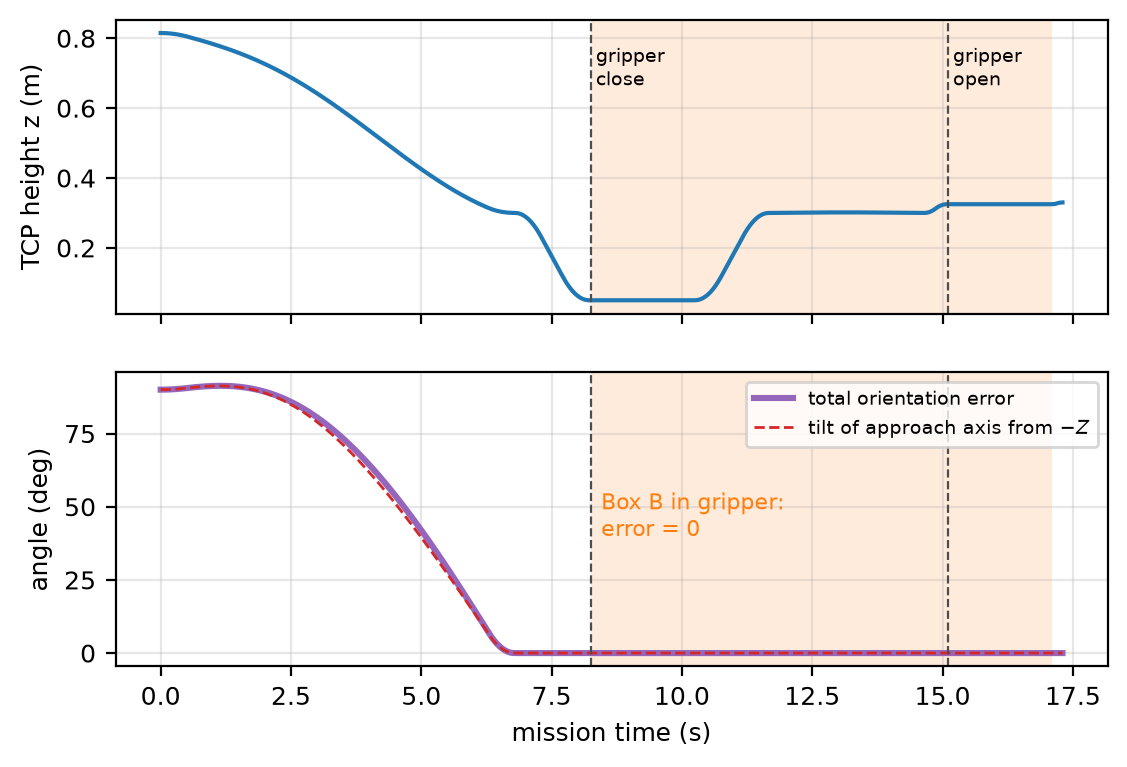
\includegraphics[width=0.78\textwidth]{mission_orientation.png}
\caption{TCP height and gripper orientation error with respect to
\(\mathbf R_\text{down}\) over the whole mission, computed by FK on the commanded
samples. Shaded: Box~B is in the gripper.}
\label{fig:orient}
\end{figure}

\subsection{LSPB velocity profile}
Each segment uses Linear Segments with Parabolic Blends (a trapezoidal velocity profile).
For the joint with the largest displacement \(|\Delta q|\) (the \emph{pacing joint}), with
velocity limit \(V_\text{max}\) and acceleration \(a\):
\begin{equation}
(t_b, t_f) =
\begin{cases}
\left(\dfrac{V_\text{max}}{a},\; \dfrac{V_\text{max}}{a} + \dfrac{|\Delta q|}{V_\text{max}}\right)
  & |\Delta q| \ge V_\text{max}^2/a \quad\text{(trapezoid)}\\[10pt]
\left(\sqrt{|\Delta q|/a},\; 2\sqrt{|\Delta q|/a}\right) & \text{otherwise (triangle)}.
\end{cases}
\end{equation}
\emph{Every} joint then uses the same \((t_b,t_f)\) with its own cruise velocity
\(V_i = \Delta q_i/(t_f - t_b)\) and blend acceleration \(a_i = V_i/t_b\):
\begin{equation}
q_i(t) =
\begin{cases}
q_{0,i} + \tfrac12 a_i t^2, & 0\le t< t_b\\
\tfrac12\big(q_{0,i}+q_{f,i} - V_i t_f\big) + V_i t, & t_b \le t \le t_f - t_b\\
q_{f,i} - \tfrac12 a_i (t_f-t)^2, & t_f - t_b < t \le t_f .
\end{cases}
\end{equation}
All joints therefore start and stop together, which gives the common-\(\sigma(t)\) property
used above. Position and velocity are continuous. Acceleration is piecewise constant
(Fig.~\ref{fig:lspb}). We use \(V_\text{max}=\SI{0.5}{rad/s}\) and
\(a=\SI{1.0}{rad/s^2}\). The profile is sampled every \(\Delta t = \SI{0.05}{s}\) and the
exact end point is appended.

\begin{figure}[h]
\centering
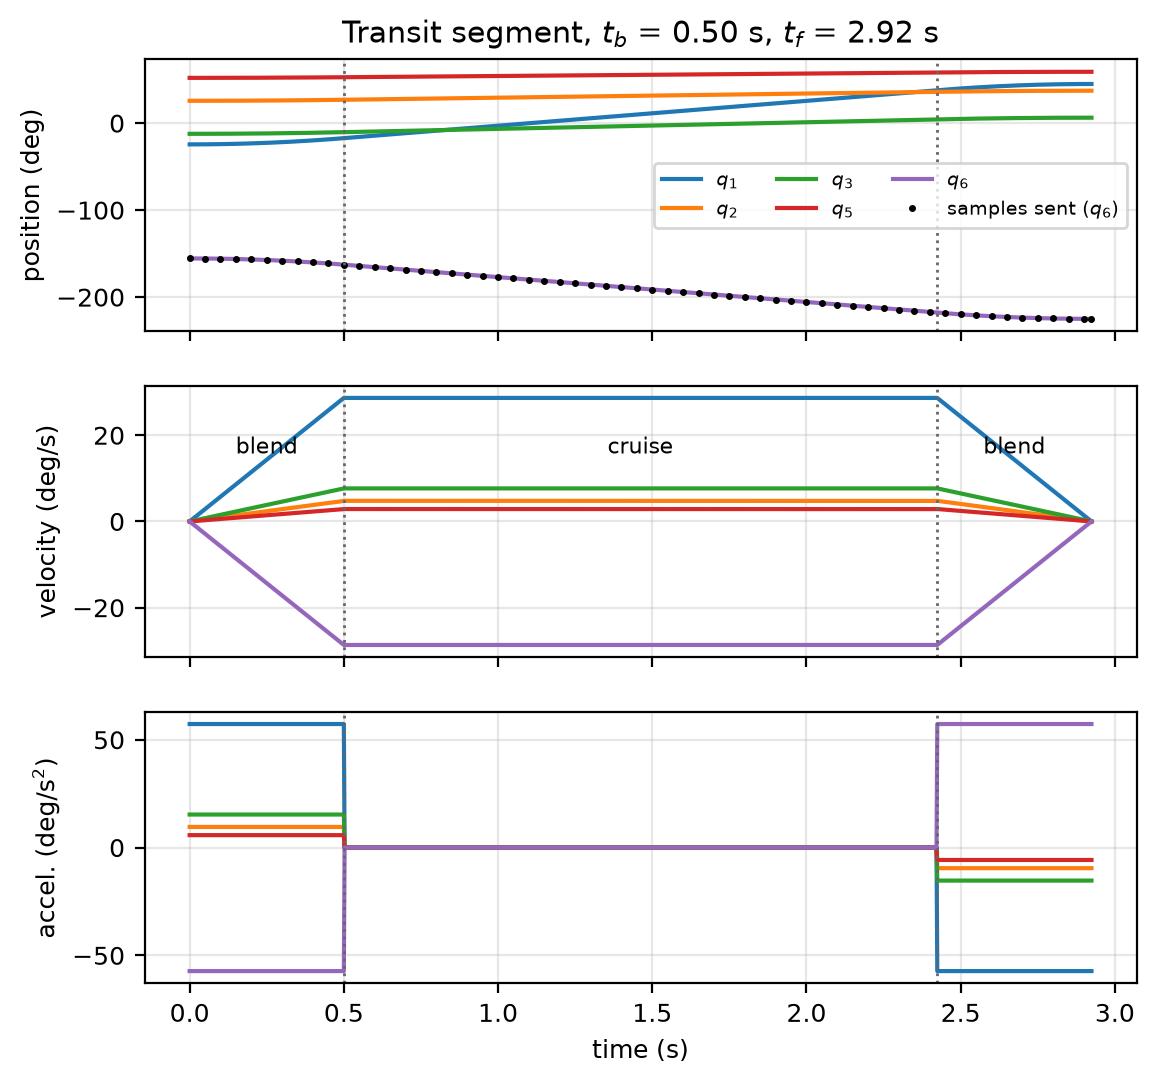
\includegraphics[width=0.74\textwidth]{lspb_transit.png}
\caption{Synchronised LSPB for the transit segment (waypoint 3\,\(\to\)\,4, Box~B held).
Joints 1 and 6 (both \(69.44^\circ\)) pace the motion. The others scale down so that all
finish at \(t_f\). Dots: the 20\,Hz samples sent to the controller. \(q_4\) does not move.}
\label{fig:lspb}
\end{figure}

\paragraph{Code: trajectory planning} (\texttt{trajectory.py}).
\lstinputlisting[firstline=4, lastline=54, firstnumber=4]{\src/trajectory.py}

% =========================================================================
\section{Velocity control}

\paragraph{Velocity limits.}
The velocity profile is what controls joint velocity. The pacing joint never exceeds
\(V_\text{max} = 0.5\,\text{rad/s} = 28.6^\circ/\text{s}\) and every other joint moves
proportionally slower. Acceleration is bounded by \(\SI{1}{rad/s^2}\). The peak commanded
speed is about 9\,\% of the slowest joint's rated speed (\(315^\circ\)/s, Table~\ref{tab:limits}).
We chose this conservative margin so that the grasped cube is not shaken loose. Short
segments (\(|\Delta q| < 14.3^\circ\)) use the triangular profile and never reach
\(V_\text{max}\).

\paragraph{Execution.}
Each segment is sent as one \texttt{FollowJointTrajectory} action goal. The goal holds the
time-stamped LSPB samples \((\mathbf q_k,\, k\Delta t)\), so the velocity profile is encoded
in the timing of the position set-points. The \texttt{JointTrajectoryController}
interpolates between samples and writes position commands to the \texttt{ros2\_control}
position interfaces at 1\,kHz. Gazebo's physics then moves the joints. The mission node
waits for each goal's result (\texttt{error\_code == SUCCESSFUL}) before it sends the next
segment or a gripper command. An earlier version polled \texttt{/joint\_states} velocities
to detect arrival. It failed because velocities are also near zero just \emph{before} a
new motion starts, so commands were sent too early. Before each gripper action, the node
reads the actual TCP pose from TF to confirm the arm is where the IK placed it.

\paragraph{Velocity kinematics.}
For analysis we also implemented the geometric Jacobian,
\(\mathbf J_{v,i} = \mathbf z_{i-1}\times(\mathbf o_6 - \mathbf o_{i-1})\) and
\(\mathbf J_{\omega,i} = \mathbf z_{i-1}\), with columns 2, 4 and 6 negated for the joint
conventions above. It matches finite-difference FK to four decimals. The manipulability
\(w=\sqrt{\det \mathbf J\mathbf J^{\mathsf T}}\) is \(0.051\)--\(0.120\) at all waypoints (smallest
singular value \(\ge 0.22\)), so the plan stays away from singularities. The home pose
\(q=0\) is a wrist singularity (\(q_5=0\), \(w=0\)). This does no harm here because the
plan is made in joint space and \(\mathbf J\) is never inverted. The other singularities
are the elbow (arm fully stretched, \(q_3 \approx 84.8^\circ\)) and the shoulder (wrist centre
on the base axis).

\paragraph{Code: velocity control and execution} (\texttt{run\_pick\_place.py}, \texttt{controllers.yaml};
logging lines omitted).
\lstinputlisting[firstline=15, lastline=40, firstnumber=15]{\src/run_pick_place.py}
\lstinputlisting[linerange={58-72,76-88,91-98}, numbers=none]{\src/run_pick_place.py}
\lstinputlisting[linerange={113-117,122-136}, numbers=none]{\src/run_pick_place.py}
\lstinputlisting[language={}, firstline=1, lastline=27]{../src/gp7_description/config/controllers.yaml}

% =========================================================================
\section{Results}

\begin{figure}[h]
\centering
\begin{subfigure}[b]{0.32\textwidth}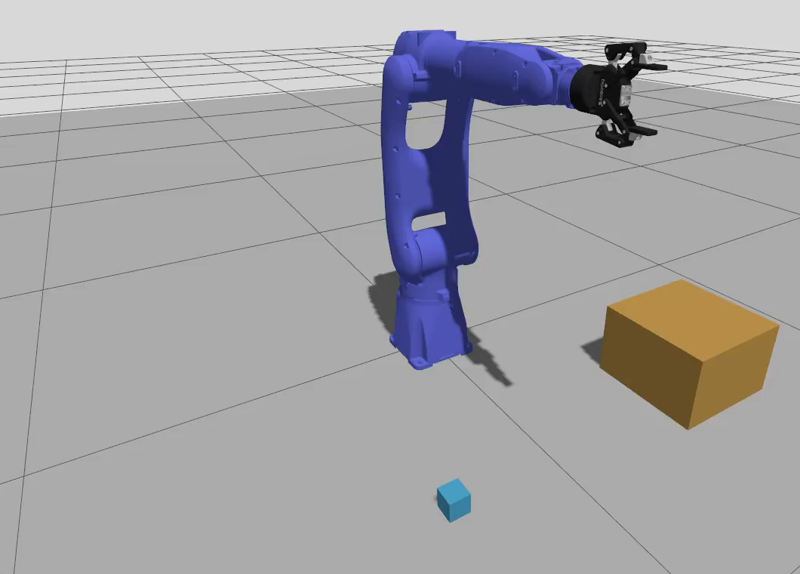
\includegraphics[width=\linewidth]{snap_0.png}\caption{start (home pose)}\end{subfigure}\hfill
\begin{subfigure}[b]{0.32\textwidth}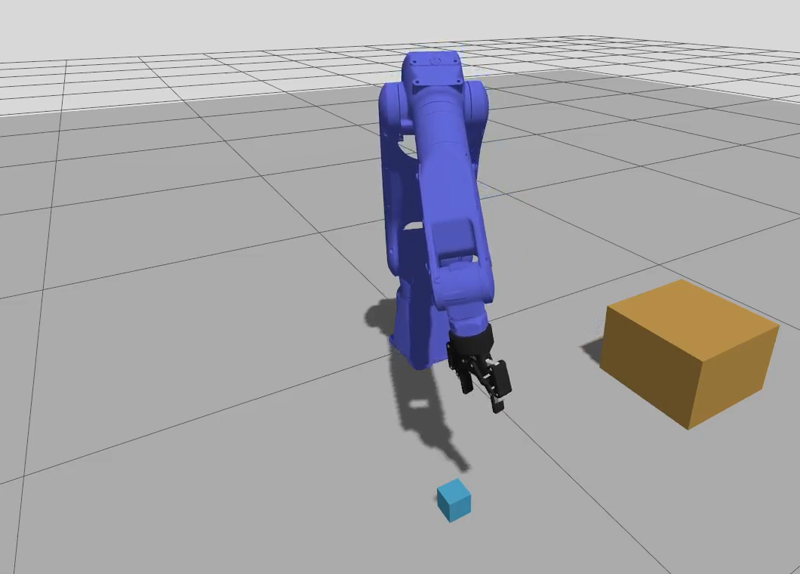
\includegraphics[width=\linewidth]{snap_10.png}\caption{descending to Box B}\end{subfigure}\hfill
\begin{subfigure}[b]{0.32\textwidth}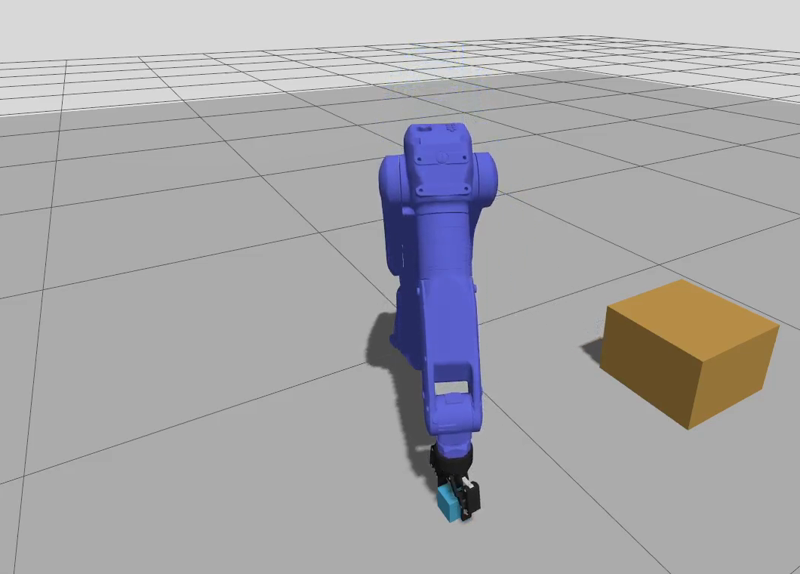
\includegraphics[width=\linewidth]{snap_12.png}\caption{grasp}\end{subfigure}\\[4pt]
\begin{subfigure}[b]{0.32\textwidth}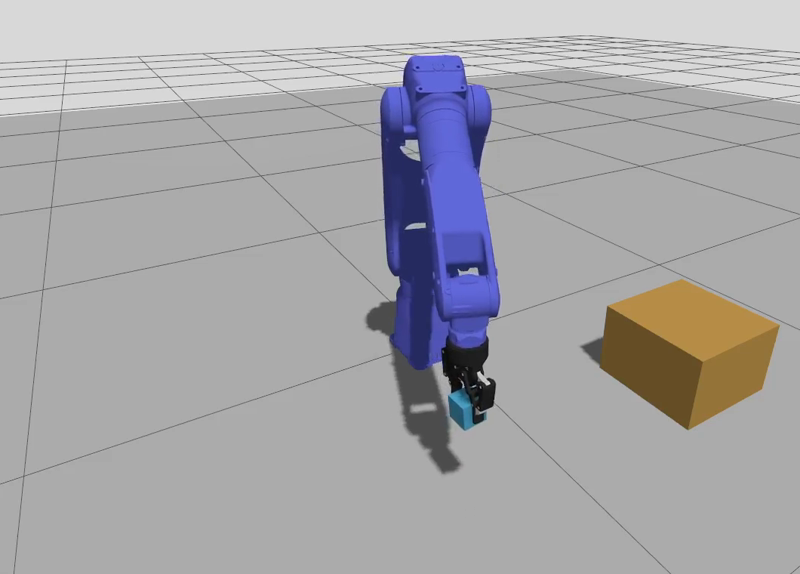
\includegraphics[width=\linewidth]{snap_16.png}\caption{transit, Box B upright}\end{subfigure}\hspace{0.02\textwidth}
\begin{subfigure}[b]{0.32\textwidth}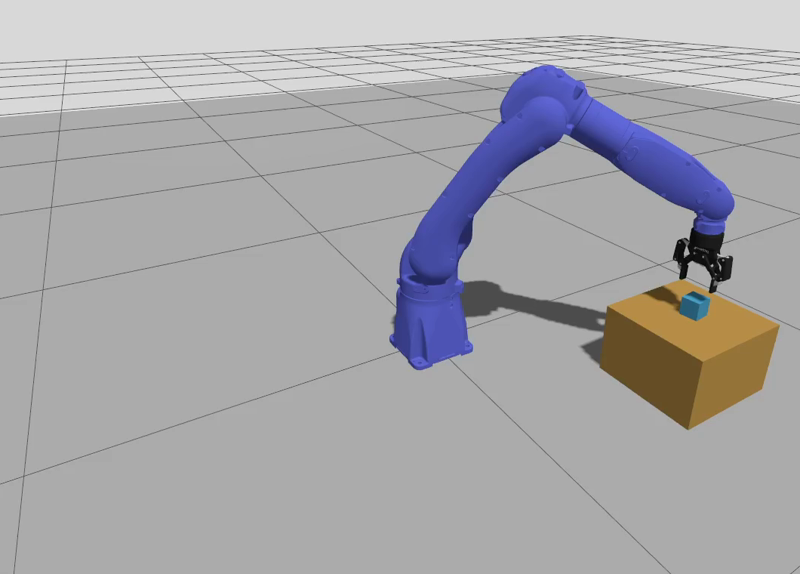
\includegraphics[width=\linewidth]{snap_21.png}\caption{placed on Box A}\end{subfigure}
\caption{Frames from the screen-recorded Gazebo run.}
\label{fig:snaps}
\end{figure}

The full sequence ran in Gazebo as planned (Fig.~\ref{fig:snaps} and the video).
Box~B was grasped, carried upright and left at the centre of Box~A's top surface. Table~\ref{tab:segments} gives the segment
timing. Arm motion takes 13.3\,s, plus two 2\,s gripper actions, for 17.3\,s in total.

\begin{table}[h]
\centering\small
\begin{tabular}{lccccc}
\toprule
Segment & Samples & Duration (s) & Pacing joint (\(|\Delta q|\)) & Profile & Path deviation \\
\midrule
home \(\to\) 1 & 137 & 6.80 & 4 (\(180^\circ\)) & trapezoid & 115\,mm \\
1 \(\to\) 2 (descend) & 30 & 1.45 & 5 (\(26.3^\circ\)) & trapezoid & 13.7\,mm \\
2 \(\to\) 3 (lift) & 30 & 1.45 & 5 (\(26.3^\circ\)) & trapezoid & 13.7\,mm \\
3 \(\to\) 4 (transit) & 60 & 2.95 & 1, 6 (\(69.4^\circ\)) & trapezoid & 121\,mm \\
4 \(\to\) 5 (lower) & 10 & 0.45 & 5 (\(2.7^\circ\)) & triangle & 0.1\,mm \\
5 \(\to\) 6 (retreat) & 5 & 0.20 & 5 (\(0.5^\circ\)) & triangle & 0.0\,mm \\
\bottomrule
\end{tabular}
\caption{Trajectory segments of the mission. Path deviation: largest distance of the TCP from the straight line joining the segment's end points.}
\label{tab:segments}
\end{table}

\paragraph{Discussion and limitations.}
\begin{itemize}
\item \textbf{Joint-space paths.} Because interpolation is in joint space, the TCP path
between waypoints is not a straight line. The vertical descent bows by
\SI{13.7}{mm}, which the 0.25\,m approach height absorbs easily. This does not affect
the box's orientation, which Section~\ref{sec:upright} shows is exactly constant.
Straight Cartesian paths would need IK at every sample or resolved-rate control.
\item \textbf{Acceleration steps.} LSPB has a continuous velocity but a discontinuous
acceleration (infinite jerk at the blend boundaries). An S-curve or quintic profile would
remove these jerk spikes.
\item \textbf{Open-loop grasp.} There is no force sensing. The gripper is commanded to a
fixed closure and friction holds the cube. The grasp and release heights were tuned
empirically, and the final retreat is only 5\,mm.
\item \textbf{No reachability error or collision checking.} The \(\arccos\) arguments are
clipped, so an unreachable target returns a stretched configuration instead of an error.
The targets were checked offline against the reach and the joint limits. There is no
obstacle avoidance.
\item \textbf{Scene change.} Box~A was moved from \((1,1,0)\) to \((0.5,0.5,0)\) because
the original position is outside the arm's reach (Section~2).
\end{itemize}

% =========================================================================
\begin{thebibliography}{9}\small
\bibitem{spong} M.~W. Spong, S.~Hutchinson, M.~Vidyasagar, \emph{Robot Modeling and Control}, 2nd ed., Wiley, 2020.
\bibitem{gp7spec} Yaskawa, \emph{Motoman GP7 robot specification sheet} (provided on Moodle).
\bibitem{rosi} ROS-Industrial, \texttt{motoman\_gp7\_support} package, \url{https://github.com/ros-industrial/motoman} (BSD licence).
\bibitem{robotiq} Robotiq, ROS description of the 2F-85 gripper, \url{https://github.com/robotiq/ros} (BSD-3-Clause).
\bibitem{dasilva} da Silva et al., ``Determination of the Inverse Kinematic of the Industrial Robot Yaskawa-Motoman-GP7,'' \emph{Advances in Robotics \& Mechanical Engineering}, 2022.
\bibitem{ros2} ROS~2 Jazzy documentation, \url{https://docs.ros.org/en/jazzy/}; \texttt{ros2\_control}, \url{https://control.ros.org}.
\bibitem{gazebo} Gazebo Harmonic documentation, \url{https://gazebosim.org/docs/harmonic}.
\end{thebibliography}

\end{document}
